\documentclass{article}

% Les packages a priori n�cessaires

\usepackage{amsmath,amssymb,amsfonts}
\usepackage{graphics}
\usepackage[T1]{fontenc}    % Accents cod�s dans la fonte.
\usepackage[latin1]{inputenc}   % Accents 8 bits dans le fichier.
\usepackage{comment} % Pour facilement enlever des inclusions � la file
\usepackage{siunitx} % Pour arrondir correctement les nombres

\usepackage[tikz]{bclogo}
\usepackage{tikz} % la base
\usetikzlibrary{calc,through,backgrounds,patterns}
\usepackage[babel=true,kerning=true]{microtype}

\usepackage{animate} % Pour faire les animations proprement dites


%%%%%%%%%%%%%%%%%%%%%%%%%%%%%%%%%%%%%%%%%%%%%
%             Les macros � JJ
%
% Quelques macros utilis�es dans mes documents
%
%%%%%%%%%%%%%%%%%%%%%%%%%%%%%%%%%%%%%%%%%%%%%

\newcommand{\bk}{\bigskip}
\newcommand{\ph}{\varphi}

\newcommand{\abs}[1]{\left|#1\right|}
\newcommand{\co}[1]{\underline{#1}}
\newcommand{\e}[1]{_{\text{#1}}}
\newcommand{\vect}[1]{\overrightarrow{#1}}

\newcommand{\f}[2]{\dfrac{#1}{#2}}


\usepackage{vmargin}
\setmarginsrb{10mm}{10mm}{10mm}{5mm}{12pt}{11mm}{0pt}{11mm}

\begin{document}

%%%%%%%%%%%%%%%%%%%%%%%%%%%%%%%%%%%%%%%%%%%%
%%%%%%%%%%%%%%%%%%%%%%%%%%%%%%%%%%%%%%%%%%%%
\section{Chapitre sur l'oscillateur harmonique}

\hfil% Dessin du ressort seul
% #1 -> longueur du ressort
% #2 -> symbole associ� ($\ell_0$ par exemple)
\newcommand{\ressort}[2]{
\pgfmathsetmacro{\taille}{1.2*#1}
\draw[ressort,decorate,decoration={coil,aspect=0.4,segment length = \taille mm,amplitude=3mm}] 
(0,-0.3)--(0,-#1) ;
\draw[thick,gray] (0,0) -- (0,-0.3); 
\fill [pattern=north east lines] (-0.5,0) rectangle (0.5,0.3); %bloc qui tient le ressort
\draw[thick] (-0.5,0) -- (0.5,0); %bloc qui tient le ressort
%fin ressort
\draw[line width=0.5pt,<->](-0.8,0) -- (-0.8,-#1) node 
[midway,left] {#2} ;
}%
% Dessin du syst�me entier
% #1 -> longueur du ressort
% #2 -> symb�le associ� ($\ell\e{�q}$ par exemple)
% #3 -> Nom de la tension ($\vect{T\e{�q}}$ par exemple)
\newcommand{\masseressort}[3]{
\ressort{#1}{#2}
\draw [rounded corners=4pt,color=white,ball color=gray,smooth] (0,{-#1-\RAYON}) circle 
(\RAYON) ;
\draw [very thick,-latex] (0,{-#1-\RAYON})--++(0,-\POIDS) node [midway,right=0cm] 
{$\vect{P}$};
\draw [very thick,-latex] (0,{-#1-0.05})--(0,{-#1 + \K*(#1-\ELLZERO)-0.05}) node [midway,right=0.25cm] 
{#3};
}
%
%
\begin{animateinline}[autoplay,loop,controls]{10}  
    \multiframe{36}{rangle=0+10}{
\begin{tikzpicture} [scale=0.75, decoration={coil,aspect=0.4,segment 
length=3mm,amplitude=3mm}]
%decoration : g�re l'aspect du ressort par l'instruction decorate
\tikzset{ressort/.style={thick,gray,smooth}} %d�finition d'un style de ressort

\draw [dashed] (2,-4.5) --++ (4,0);
\draw node [left] at (2,-4.5) {O}; 
\draw [->] (2,-6.5) --++ (0,3) node [left] {$z$};
\draw [dashed] (2,-5.5) --++ (4,0) ;
\draw node [left] at (2,-5.5) {ici $z(t)<0$} ;

\pgfmathsetmacro{\ELLZERO}{2.2}
\pgfmathsetmacro{\ELLEQ}{4.1}
\pgfmathsetmacro{\AMPLITUDE}{1}
\pgfmathsetmacro{\RAYON}{0.4}
\pgfmathsetmacro{\POIDS}{1.5}
\pgfmathsetmacro{\K}{\POIDS / (\ELLEQ-\ELLZERO)}
\pgfmathsetmacro{\ELL}{\ELLEQ + \AMPLITUDE*cos(\rangle)}


% ressort seul
\begin{scope}
\ressort{\ELLZERO}{$\ell_0$}
\end{scope}

% Syst�me entier � l'�quilibre
\begin{scope}[xshift=3cm]%D�calage horizontale de 3 cm
\masseressort{\ELLEQ}{$\ell\e{�q}$}{$\vect{T\e{�q}}$}
\end{scope}

% Syst�me entier en mouvement
\begin{scope}[xshift=6cm]
\masseressort{\ELL}{$\ell(t)$}{$\vect{T}$}
\end{scope}

% L�gendes
\begin{scope}[xshift=-1cm,yshift=-5.5cm]
\draw [rounded corners=4pt,color=white,ball color=gray,smooth] (0,-2.5) circle 
(0.4) node [right=0.75cm,black] {: objet M de masse $m$} ;
\draw[ressort,decorate,rotate=0] (-0.75,-3.5)--(0.75,-3.5) node 
[right=0cm,black] {: ressort de constante de raideur $k$};
\end{scope}
\end{tikzpicture}
    }
\end{animateinline}





\bk

\hfil\begin{animateinline}[autoplay,loop,controls]{10}
    \multiframe{36}{rangle=0+10}{
\begin{tikzpicture} [scale=0.75, decoration={coil,aspect=0.4,segment 
length=3mm,amplitude=3mm}]
%decoration : g�re l'aspect du ressort par l'instruction decorate
\tikzset{ressort/.style={thick,gray,smooth}} %d�finition d'un style de ressort

\draw [dashed] (4.5,2) --++ (0,-8);
\draw node [above] at (4.5,2) {O}; 
\draw [->] (0,2) --++ (7,0) node [above] {$x$};

\pgfmathsetmacro{\ELLZERO}{4.5}
\pgfmathsetmacro{\AMPLITUDE}{1.3}
\pgfmathsetmacro{\ELLUP}{  \ELLZERO - \AMPLITUDE*cos(\rangle)}
\pgfmathsetmacro{\ELLDOWN}{\ELLZERO + \AMPLITUDE*cos(\rangle)}
\pgfmathsetmacro{\K}{3}


%\newcommand{\ellmacro}[1]{
%\ifthenelse{\equal{#1}{\ELLZERO}}{\ell_0}{\ell(t)}
%}

% #1 -> la longueur du ressort
% #2 -> \ell_0 ou \ell(t)
\newcommand{\systemeMasseRessort}[3]{

%bloc qui tient le ressort 
\draw[thick,gray] (0,0) -- (0.3,0); 
\fill [pattern=north east lines] (0,0.5) rectangle (-0.3,-0.5); 
%pattern d�finit un style de remplissage de la forme
\draw[thick](0,0.5)--(0,-0.5); %fin ressort
% Le ressort proprement dit
\pgfmathsetmacro{\taille}{1.2*#1}
\draw[ressort,decorate,decoration={coil,aspect=0.62,segment length = \taille mm,amplitude=3mm}] 
(0.3,0)--(#1,0) ;
% La l�gende au-dessus
\draw[line width=0.5pt,<->](0,+0.8) -- (#1,+0.8) node [midway,above] {$#2$} ;
% La masse
\draw [rounded corners=4pt,color=white,ball color=gray,smooth] (#1,-0.5) rectangle ({#1+1},0.5);
\draw[thick](2,-0.5)--(7.3,-0.5); %fin du plancher
\fill [pattern=north east lines] (2,-0.5) rectangle (7.3,-0.8); 
\draw [very thick,-latex] ({#1+0.5},0)--++(0,-1.5) node [right] {$\vect{P}$};
\draw [very thick,-latex] ({#1+0.6},-0.5)--++(0,1.5) node [right] {$\vect{N}$};
% Si on est � \ell_0, pas de fl�che, sinon on la marque
\ifthenelse{\equal{#1}{\ELLZERO}}{
\draw (#1,0) node [above] {$#3$} ;
}{
\draw [very thick,-latex] (#1,0)--++({-\K*(#1-\ELLZERO)},0) node [midway,above] {$\vect{T}$};
}
}


\begin{scope}[yshift=0cm]
\systemeMasseRessort{\ELLUP}{\ell(t)}{\vect{T}}
\end{scope}

\begin{scope}[yshift=-3cm]
\systemeMasseRessort{\ELLZERO}{\ell_0}{}
\end{scope}

\begin{scope}[yshift=-6cm]
\systemeMasseRessort{\ELLDOWN}{\ell(t)}{\vect{T}}
\end{scope}
\end{tikzpicture}
}
\end{animateinline}



%%%%%%%%%%%%%%%%%%%%%%%%%%%%%%%%%%%%%%%%%%%%
%%%%%%%%%%%%%%%%%%%%%%%%%%%%%%%%%%%%%%%%%%%%
\section{Chapitre sur les ondes}

L'utilisation d'une cinquantaine d'image a tendance � alourdir 
consid�rablement le fichier pdf produit (ce qui est, somme toute, assez 
logique). Si vous voulez voir ces animations, il vous faudra t�l�charger le 
projet et enlever l'environnement \texttt{\{comment\}} plac� autour d'elles 
avant de recompiler le document sur votre propre machine (vous feriez 
mieux d'inclure le fichier idoine dans le fichier \texttt{minimal.tex} car la 
compilation du document complet est tr�s longue).

\begin{comment}
\hfil\animategraphics[controls,width=0.7\linewidth]{4}{PNG/S02_dualite_temporel_spatial_droite_}{00}{49}


\bk

\hfil\animategraphics[controls,width=0.7\linewidth]{4}{PNG/S02_dualite_temporel_spatial_gauche_}{00}{49}


\bk

\hfil\animategraphics[controls,loop,width=0.6\linewidth]{10}{PNG/S04_onde_EM_}{00}{49}


\bk

\hfil\animategraphics[width=0.8\linewidth,controls,palindrome]{4}{PNG/S03_diffraction_anim_}{0000}{0019}


\end{comment}

%%%%%%%%%%%%%%%%%%%%%%%%%%%%%%%%%%%%%%%%%%%%
%%%%%%%%%%%%%%%%%%%%%%%%%%%%%%%%%%%%%%%%%%%%
\section{Chapitre oscillateurs amortis}

\hfil\begin{animateinline}[autoplay,loop,controls,poster=last]{10}
    \multiframe{33}{rangle=00+30}{
\begin{tikzpicture}[scale=0.75, decoration={coil,aspect=0.4,segment 
length=3mm,amplitude=3mm}, 
declare function = {
longueur(\x) = 3 + cos(\x)*exp(-1*\x/360) ;
altitude(\x) = 2.0 - longueur(\x) ; 
}]
\tikzset{ressort/.style={thick,gray,smooth}}
\pgfmathsetmacro{\A}{1.0}
\pgfmathsetmacro{\taille}{1.1*longueur(\rangle)}
\begin{scope}[xshift=0cm]
%ressort 
\draw[ressort,decorate,decoration={segment length=\taille mm}] (0,2) --(0,{altitude(\rangle)}) ;
\fill [pattern=north east lines] (-0.5,3.7) rectangle (0.5,4.0);
\draw[thick,gray] (-0.5,3.7) -- (0.5,3.7);
\draw[thick,gray] (0,3.7) -- (0,2); 
\draw [thick, gray] (0,{altitude(\rangle)})--(0,{altitude(\rangle)-0.7});
\draw [color=white,ball color=gray,smooth] (0,{altitude(\rangle)-0.7}) circle (0.4) node 
[black,below right=0.2cm] {\scriptsize{M}} ;
%fin ressort 

%eprouvette 
\draw [gray,very thick] (-1,-4) --++ (0,5);
\draw [gray,very thick] (1,-4) --++ (0,5);
\draw [gray,very thick] (-2,-4) --++ (4,0);
\fill [gray,opacity=0.2] (-1,-4) rectangle (1,0);
%fin eprouvette 

%g�n�rateur 
\draw (3,-3.3) rectangle++ (3,1.5) node [midway, above=0.1cm] {G�n�rateur};
\draw [black] (5.2,-2.7) circle (0.1cm) node [below=0.025cm] 
{\scriptsize{Masse}};
\filldraw [black] (3.8,-2.7) circle (0.1cm) node [below=0.025cm] 
{\scriptsize{+}};
% fin g�n�rateur 

%oscilloscope 
\draw (3,-1) rectangle++ (3,2) node [midway, above=0.1cm] {Oscilloscope};
\draw node at (3.7,-0.7) {\scriptsize{Voie 1}};
\filldraw [black] (3.4,-0.3) circle (0.1cm);
\draw [black] (4,-0.3) circle (0.1cm);
%fin oscilloscope 

%fils 
\draw [red] (3.8,-2.7) --++ (-2,0) --++ (0,4) --++ (-1.1,0) --++ (0,-1.5);
\draw [black] (5.2,-2.7) --++ (1.5,0) --++ (0,-1.75) --++ (-9,0) --++ (0,5.75) 
--++ (1.6,0) --++ (0,-5);

\filldraw [black] (-0.85,-3.8) rectangle++ (0.3,0.1) node [right] 
{\scriptsize{B}};
\filldraw [red] (0.55,-0.2) rectangle++ (0.3,0.1) node [below] at (0.7,-0.2) 
{\scriptsize{A}};

\draw [red] (3.4,-0.3) --++ (-0.7,0) --++ (0,3) --++ (-2.7,0) node [left, 
black] {\scriptsize{M'}};
\draw [black] (4,-0.3) --++ (2.7,0) --++ (0,-2.4);

%fin fils 

\end{scope}
\begin{scope}[xshift=8cm]
\draw [smooth,ultra thick,domain=0:{\rangle/180},samples={1+\rangle/10}] plot (\x,{altitude(\x*180)-0.7}) ;
\draw [thick,->] ({-2pt},-3.75) -- ({1100/180},-3.75) node [above] {$t$}; 
\draw [thick,->] (0,{-3.8}) -- (0,1) node [right] {$u_{AB}(t)$} ;
\end{scope}
\end{tikzpicture}
}
\end{animateinline}



\bk

\hfil\begin{animateinline}[autoplay,loop,controls,poster=last]{10}
    \multiframe{33}{rangle=00+30}{
\begin{tikzpicture}[scale=0.75, decoration={coil,aspect=0.4,segment 
length=3mm,amplitude=3mm}, 
declare function = {
solution(\x,\A,\B) = (\A*exp(-\rU*\x/360) + \B*exp(-\rD*\x/360))*2 ;
vitesse(\x,\A,\B)  = (-\rU*\A*exp(-\rU*\x/360) - \rD*\B*exp(-\rD*\x/360))/3 ;
}]
\tikzset{ressort/.style={thick,gray,smooth}}
\pgfmathsetmacro{\rU}{2}
\pgfmathsetmacro{\rD}{3}
\begin{scope}[xshift=0cm]
%\draw (4,3.5) node {Amortissement fort} ;
\draw [->,thick] (0,-3) -- (0,3) node [right] {$\dot{z}$};
\draw [->,thick] (-3,0) -- (3,0) node [above] {$z$} ;
\draw [smooth,ultra thick,domain=0:{\rangle/180},samples={1+\rangle/30},variable=\x] plot
({solution(\x*180,5,-5)},{vitesse(\x*180,5,-5)}) ;
\draw [smooth,ultra thick,dashed,domain=0:{\rangle/180},samples={1+\rangle/30},variable=\x] plot
({solution(\x*180,\rD,-\rU)},{vitesse(\x*180,\rD,-\rU)}) ;
%\draw [smooth,ultra thick,dotted,domain=0:{\rangle/180},samples={1+\rangle/30},variable=\x] plot
%({solution(\x*180,-\rD,2*\rU)},{vitesse(\x*180,-\rD,2*\rU)}) ;
\draw [smooth,dotted,ultra thick,domain=0:{\rangle/180},samples={1+\rangle/30},variable=\x] plot
({solution(\x*180,-5,5.5)},{vitesse(\x*180,-5,5.5)}) ;


\end{scope}
\begin{scope}[xshift=8cm]
\draw [smooth,ultra thick,domain=0:{\rangle/180},samples={1+\rangle/30}] plot 
(\x,{solution(\x*180,5,-5)}) ;
\draw [smooth,dotted,ultra thick,domain=0:{\rangle/180},samples={1+\rangle/30}] plot 
(\x,{solution(\x*180,-5,5.5)}) ;
\draw [smooth,ultra thick,dashed,domain=0:{\rangle/180},samples={1+\rangle/30}] plot 
(\x,{solution(\x*180,\rD,-\rU)}) ;
\draw [->,thick] ({-2pt},0) -- ({1100/180},0) node [above] {$t$}; 
\draw [->,thick] (0,{-3}) -- (0,3) node [right] {$z(t)$} ;
\end{scope}
\end{tikzpicture}
}
\end{animateinline}



\bk

\hfil\begin{animateinline}[final,autoplay,loop,controls,poster=last]{5}
    \multiframe{33}{rangle=00+30}{
\begin{tikzpicture}[scale=0.75, decoration={coil,aspect=0.4,segment 
length=3mm,amplitude=3mm}, 
declare function = {
solution(\x,\A,\B) = (exp(-\LAMBDA*\x/360)*(\A*cos(\OMEGA*\x) + \B*sin(\OMEGA*\x))/2 ;
%vitesse(\x,\A,\B)  = (exp(-\LAMBDA*\x/360)*((\B*\OMEGA*\CORRO-\A*\LAMBDA*\CORRL)*cos(\OMEGA*\x) - (\A*\OMEGA*\CORRO+\B*\LAMBDA*\CORRL)*sin(\OMEGA*\x))/10 ;
vitesse(\x,\A,\B)  = (exp(-\LAMBDA*\x/360)*((\B*\OMEGA-\A*\LAMBDA/360)*cos(\OMEGA*\x) - (\A*\OMEGA+\B*\LAMBDA/360)*sin(\OMEGA*\x))/2 ;
}]
\tikzset{ressort/.style={thick,gray,smooth}}
\pgfmathsetmacro{\LAMBDA}{2}
\pgfmathsetmacro{\OMEGA}{1}
\pgfmathsetmacro{\CORRO}{3.14159/180}
\pgfmathsetmacro{\CORRL}{3.14159*2}
\begin{scope}[xshift=0cm]
%\draw (4,3.5) node {Amortissement fort} ;
\draw [->,thick] (0,-3) -- (0,3) node [right] {$\dot{z}$};
\draw [->,thick] (-3,0) -- (3,0) node [above] {$z$} ;
\draw [smooth,ultra thick,domain=0:{\rangle/180},samples={1+\rangle/10},variable=\x] plot
({solution(\x*180,0,4)},{vitesse(\x*180,0,4)}) ;
\draw [smooth,ultra thick,dashed,domain=0:{\rangle/180},samples={1+\rangle/10},variable=\x] plot
({solution(\x*180,5,-5)},{vitesse(\x*180,5,-5)}) ;
\draw [smooth,dotted,ultra thick,domain=0:{\rangle/180},samples={1+\rangle/10},variable=\x] plot
({solution(\x*180,4,0)},{vitesse(\x*180,4,0)}) ;


\end{scope}
\begin{scope}[xshift=8cm]
\draw [smooth,ultra thick,domain=0:{\rangle/180},samples={1+\rangle/30}] plot 
(\x,{solution(\x*180,0,4)}) ;
\draw [smooth,dotted,ultra thick,domain=0:{\rangle/180},samples={1+\rangle/30}] plot 
(\x,{solution(\x*180,4,0)}) ;
\draw [smooth,ultra thick,dashed,domain=0:{\rangle/180},samples={1+\rangle/30}] plot 
(\x,{solution(\x*180,5,-5)}) ;
\draw [->,thick] ({-2pt},0) -- ({1100/180},0) node [above] {$t$}; 
\draw [->,thick] (0,{-3}) -- (0,3) node [right] {$z(t)$} ;
\end{scope}
\end{tikzpicture}
}
\end{animateinline}




%%%%%%%%%%%%%%%%%%%%%%%%%%%%%%%%%%%%%%%%%%%%
%%%%%%%%%%%%%%%%%%%%%%%%%%%%%%%%%%%%%%%%%%%%
\section{Chapitre oscillateurs forc�s}

\hfil%
\begin{animateinline}[autoplay,loop,controls]{10}  
    \multiframe{36}{rangle=180+10}{
\begin{tikzpicture}[scale=0.75, decoration={coil,aspect=0.4,segment
length=3mm,amplitude=3mm}]
\pgfmathsetmacro{\amplitude}{1}
\pgfmathsetmacro{\A}{0.28}
\pgfmathsetmacro{\longueur}{3 + \A*cos(\rangle) - \amplitude*sin(\rangle)}
\pgfmathsetmacro{\taille}{1.1*\longueur}
%ressort
\tikzset{ressort/.style={thick,gray,smooth}}
\begin{scope}[xshift=5cm]
\draw[ressort,decorate,decoration={segment length=\taille mm}] (0.3,{2+\A*cos(\rangle)})--(0.3,{-1+\amplitude*sin(\rangle)}) ;   
\fill [pattern=north east lines] (-0.5,4.2) rectangle (0.5,4.5); %bloc qui 
tient le ressort
\draw[thick,gray] (-0.5,4.2) -- (0.5,4.2); %bloc qui tient le ressort
\draw[thick,gray] (0.3,3.7) -- (0.3,{2+\A*cos(\rangle)}); %tige au dessus ressort
\draw[thick,gray] (0,4.2) -- (0,3.9);
%fin ressort
\end{scope}
\draw (0,-2) rectangle (2,-0.5) node [midway, above=0.15cm ] {Moteur};
\draw (5,3.6) circle (0.28cm);
\draw (1.5,-1.5) circle (0.28cm);
\filldraw [black] ({1.5+0.28*cos(\rangle-135)},{-1.5+0.28*sin(\rangle-135)}) circle (0.08cm);
\draw [gray] ({1.5+0.28*cos(\rangle-135)},{-1.5+0.28*sin(\rangle-135)}) -- (4.7,3.7);
\draw [thick, gray] (5.3,{-1+\amplitude*sin(\rangle)})--(5.3,{-1.9+\amplitude*sin(\rangle)});
\draw [color=white,ball color=gray,smooth] (5.3,{-1.7+\amplitude*sin(\rangle)}) circle (0.4) ;
%eprouvette rempli de solution
\draw [gray, very thick] (4.6,-4) --++ (0,5);
\draw [gray, very thick] (6.0,-4) --++ (0,5);
\draw [gray, very thick] (3.6,-4) --++ (3.4,0);
\fill [gray,opacity=0.2] (4.6,-4) rectangle (6.0,0);
%fin eprouvette
\end{tikzpicture}
}
\end{animateinline}


\bk

\hfil\begin{animateinline}[final,autoplay,loop,controls,poster=last]{1}
    \multiframe{5}{iCOUNT=1+1}{
\begin{tikzpicture}[scale=0.75]
\pgfmathsetmacro{\AUN}{2.0}
\pgfmathsetmacro{\ADEUX}{4}
\pgfmathsetmacro{\PHI}{60}
\pgfmathsetmacro{\ATOT}{sqrt(\AUN^2+\ADEUX^2+2*\AUN*\ADEUX*cos(\PHI))}
\pgfmathsetmacro{\PHITOT}{acos(-(\ADEUX^2 - \AUN^2 - \ATOT^2)/(2*\AUN*\ATOT) ) }
\pgfmathsetmacro{\HMAX}{4.5}
\draw [->,thick] (0,-10pt) -- (0,\HMAX) ;
\draw [->,thick] (-10pt,0) -- (\HMAX,0) ;
\draw [->,ultra thick] (0,0) -- (\AUN,0) node [pos=0.5,below] {$A_1$};
\ifthenelse{\iCOUNT > 1}{
  \draw [->,ultra thick] (0,0) -- ({\ADEUX*cos(\PHI)},{\ADEUX*sin(\PHI)}) node [pos=0.5,above left=-2pt] {$A_2$};
  \ifthenelse{\iCOUNT < 4}{
    \draw [->,thick] (0.4,0) arc (0:\PHI:0.4) node [right] {$\ph$} ;
  }{}
  \ifthenelse{\iCOUNT > 2}{
    \draw [very thick,dashed] ({\ADEUX*cos(\PHI)},{\ADEUX*sin(\PHI)}) --++ (\AUN,0) node [pos=0.5,above] {$A_1$};
    \draw [very thick,dashed] (\AUN,0) --++ ({\ADEUX*cos(\PHI)},{\ADEUX*sin(\PHI)}) node [pos=0.5,below right=-2pt] {$A_2$};
    \draw [->,thick] ({\AUN+0.4},0) arc (0:\PHI:0.4) node [right] {$\ph$} ;
  }{}
  \ifthenelse{\iCOUNT > 3}{
    \draw [->,ultra thick] (0,0) -- ({\ADEUX*cos(\PHI)+\AUN},{\ADEUX*sin(\PHI)}) node [pos=0.75,above left=-2pt] {$A\e{tot}$};
    \draw [->,ultra thick] (0.6,0) arc (0:\PHITOT:0.6) node [right] {$\ph\e{tot}$} ;
  }{}
}{}
\end{tikzpicture}
}
\end{animateinline}



\bk

\hfil\begin{animateinline}[final,autoplay,loop,controls,poster=last,palindrome]{5}
    \multiframe{20}{rOMEGA=0.1+0.1}{
\begin{tikzpicture}[scale=0.75, decoration={coil,aspect=0.4,segment 
length=3mm,amplitude=3mm}, 
declare function = {
H(\x) = 1 /(sqrt((\Q*(\x - 1/\x))^2 + 1)) ;
phi(\x) = -atan(\Q * (\x - 1/\x)) ;
uL(\x)  = \Q * \x ;
uC(\x)  = \Q / \x ;
}]
\pgfmathsetmacro{\Q}{2}
\begin{scope}[xshift=0cm]
%\draw (4,3.5) node {Amortissement fort} ;
\clip (-4.5,-4.5) rectangle (4.5,5.5) ;
\draw [->,thick] (0,-4) -- (0,4.5) node [left] {$\Im(\co{u})$};
\draw [->,thick] (-1,0) -- (3,0) node [above] {$\Re(\co{u})$};
\draw [->,ultra thick] (0,0) -- (0,{uL(\rOMEGA)})   node [left]  {$\co{u}_L$} ;
\draw [->,ultra thick] (0,{uL(\rOMEGA)}) --++ (1,0) node [above] {$\co{u}_R$} ;
\draw [->,ultra thick] (1,{uL(\rOMEGA)}) --++ (0,{-uC(\rOMEGA)}) node [right] {$\co{u}_C$} ;
\draw [->,ultra thick] (0,0) -- (1,{uL(\rOMEGA)-uC(\rOMEGA)})   node [pos=0.5,above]  {$\co{E}$} ;
\draw [->,thick] (0.4,0) arc (0:{int(0-phi(\rOMEGA))}:0.4) node [right] {\small$-\ph$} ;
\end{scope}
\begin{scope}[xshift=4cm]
%\draw [ultra thick, domain=0.1:2, samples={\rOMEGA/0.1*2+1}] plot (\x,{H(\x)*2}) ;
\draw [ultra thick,domain=0.1:2,samples=100] plot (2*\x,{H(\x)*3} ) ;
\draw [->,thick] (-10pt,0) -- (4.5,0) node [above] {$\omega$} ;
\draw [->,thick] (0,-10pt) -- (0,4.5) node [right] {$A(\omega)=\abs{\co{u}_R}/\abs{\co{E}}$} ;
\draw [dashed,thick] (2,0) node [below] {$\omega_0$} --++ (0,3) --++ (-2,0) node [left] {$1$} ; 
\filldraw [black] ({2*\rOMEGA},{3*H(\rOMEGA)}) circle (2pt) ;
\draw (1,-2) node [left] {$\omega=\rOMEGA\,\omega_0$} ;
\end{scope}
\begin{scope}[xshift=10cm]
%\draw [ultra thick, domain=0.1:2, samples={\rOMEGA/0.1*2+1}] plot (\x,{H(\x)*2}) ;
\draw [ultra thick,domain=0.1:2,samples=100] plot (2*\x,{phi(\x)/180*5} ) ;
\draw [->,thick] (-10pt,0) -- (4.5,0) node [above] {$\omega$} ;
\draw [->,thick] (0,-4) -- (0,4.5) node [right] {$\ph(\omega)$} ;
\filldraw [black] ({2*\rOMEGA},{phi(\rOMEGA)/180*5}) circle (2pt) ;
\draw [dashed,thick] (0,2.5) node [left] {$\pi/2$} -- (4,2.5) ;
\draw [dashed,thick] (0,-2.5) node [left] {$-\pi/2$} -- (4,-2.5) ;
\end{scope}
\end{tikzpicture}
}
\end{animateinline}



\bk

\hfil\sisetup{round-mode=places,round-precision=1}
\begin{animateinline}[final,autoplay,controls,poster=last]{1}
    \multiframe{10}{iCOUNT=1+1}{
\begin{tikzpicture}[declare function = {
module(\x) = \E / sqrt((1-(\x/\fZ)^2)^2 + (\x/(\Q*\fZ))^2) ;
phase(\x)  = (0-90 - atan(\Q*(\x/\fZ - \fZ/\x)))/60 ;
}]

\pgfmathsetmacro{\Q}{1.2}
\pgfmathsetmacro{\E}{3}
\pgfmathsetmacro{\fZ}{2.2}
\pgfmathsetmacro{\fMAX}{3.1*\fZ}
\pgfmathsetmacro{\zMAX}{1.2*\Q*\E}

\draw [help lines] (0,0) grid ({\fMAX},{\Q*\E*1.2}) ;
\draw [->,thick] (-10pt,0) -- ({\fMAX},0) node [below right] {$f$ (Hz)}   ;
\draw [->,thick] (0,-10pt) -- (0,{\zMAX}) node [above left] {$u_0$ (V)};
\draw [mark=*,only marks,domain=0:{\fMAX},samples=15] plot (\x,{module(\x)}) ;

\pgfmathsetmacro{\FIN}{int(\fMAX)}
\foreach \x in {1,2,...,\FIN} {
    \pgfmathsetmacro{\y}{int(10*\x)}
    \draw (\x,0) node [below] {$\y$} ;
}

\pgfmathsetmacro{\FIN}{int(\zMAX)}
\foreach \x in {1,2,...,\FIN} {
    \draw (0,\x) node [left] {$\x$} ;
}

\begin{scope}[blue]
\ifthenelse{\iCOUNT > 5}{
  \draw [fill] (0,\E) circle (3pt);
  \draw (1,\zMAX) node [above] {$E_0=\E$}  ;
  \ifthenelse{\iCOUNT > 6}{
    \draw [domain=0:{\fMAX},samples=50] plot (\x,{module(\x)}) ;
    \ifthenelse{\iCOUNT > 7}{
      \draw [dashed,thick] (\fZ,0) -- (\fZ,{\Q*\E}) ;
      \draw [fill] (\fZ,{\Q*\E}) circle (2pt) ;
      \ifthenelse{\iCOUNT > 8}{
        \pgfmathsetmacro{\y}{\Q*\E}
        \draw [dashed,thick] (\fZ,{\Q*\E}) --++ (-\fZ,0) ;
        \draw (3,\zMAX) node [above] {$QE_0=\num{\y}$} ;
        \ifthenelse{\iCOUNT > 9}{
          \draw (6,\zMAX) node [above=-4pt] {donc $\boxed{Q=\Q}$} ;
        }{}
      }{}
    }{}
  }{}
}{}
\end{scope}

\begin{scope}[shift={(\fMAX+1.5,3)}]
%\draw (0,0) circle (2mm) ;
\draw [->,thick](0,0) -- (\fMAX,0) node [above right] {$f$ (Hz)} ;
\draw [->,thick](0,-3) -- (0,1.3) node [above right] {$\ph$ (degr�)} ;
\draw [help lines] (0,1) grid (\fMAX,-3) ;
\draw [mark=*,only marks,domain=0.001:{\fMAX},samples=15] plot (\x,{phase(\x)}) ;

\pgfmathsetmacro{\FIN}{int(\fMAX)}
\foreach \x in {1,2,...,\FIN} {
    \pgfmathsetmacro{\y}{int(10*\x)}
    \draw (\x,0) node [above] {$\y$} ;
}
\foreach \x in {1,0,...,-2} {
    \pgfmathsetmacro{\y}{int(60*\x)}
    \draw (0,\x) node [left] {$\y$} ;
}

\begin{scope}[blue]
\ifthenelse{\iCOUNT > 1}{
  \draw [domain=0.001:{\fMAX},samples=50] plot (\x,{phase(\x)}) ;
}{}
\ifthenelse{\iCOUNT > 2}{
  \draw (0,-1.5) node [left] {$-90$} ;
  \ifthenelse{\iCOUNT > 3}{
    \draw [dashed,thick] (0,-1.5) -- (\fZ,-1.5) ;
    \draw [fill] (\fZ,-1.5) circle (2pt) ;
    \ifthenelse{\iCOUNT > 4}{
      \pgfmathsetmacro{\y}{int(round(\fZ*10))}
      \draw [dashed,thick] (\fZ,-1.5) -- (\fZ,1.2) node [above right=-4pt] {\fbox{$f_0=\y$ Hz}} ;
    }{}
  }{}
}{}
\end{scope}
\end{scope}
\end{tikzpicture}
}
\end{animateinline}


\bk

\hfil\sisetup{round-mode=places,round-precision=1}
\begin{animateinline}[final,autoplay,controls,poster=last]{1}
    \multiframe{15}{iCOUNT=1+1}{
\begin{tikzpicture}[declare function = {
module(\x) = \E*(\x/(\Q*\fZ)) / sqrt((1-(\x/\fZ)^2)^2 + (\x/(\Q*\fZ))^2) ;
phase(\x)  = (0-atan(\Q*(\x/\fZ - \fZ/\x)))/60 ;
}]

\pgfmathsetmacro{\Q}{1.2}
\pgfmathsetmacro{\E}{3}
\pgfmathsetmacro{\fZ}{2.2}
\pgfmathsetmacro{\fMAX}{3.1*\fZ}
\pgfmathsetmacro{\zMAX}{\Q*\E*1.2}
\pgfmathsetmacro{\zECRIT}{\zMAX+0.2}
\pgfmathsetmacro{\zSTEP}{0.7}
\pgfmathsetmacro{\fUN}  {\fZ * (sqrt(1 + 1/(4*\Q^2)) - 1/(2*\Q)))}
\pgfmathsetmacro{\fDEUX}{\fZ * (sqrt(1 + 1/(4*\Q^2)) + 1/(2*\Q)))}


\draw [help lines] (0,0) grid ({\fMAX},{\zMAX}) ;
\draw [->,thick] (-10pt,0) -- ({\fMAX},0) node [below right] {$f$ (Hz)}   ;
\draw [->,thick] (0,-10pt) -- (0,{\zMAX}) node [above left] {$u_0$ (V)};
\draw [mark=*,only marks,domain=0:{\fMAX},samples=15] plot (\x,{module(\x)}) ;

\pgfmathsetmacro{\FIN}{int(\fMAX)}
\foreach \x in {1,2,...,\FIN} {
    \pgfmathsetmacro{\y}{int(10*\x)}
    \draw (\x,0) node [below] {$\y$} ;
}

\pgfmathsetmacro{\FIN}{int(\zMAX)}
\foreach \x in {1,2,...,\FIN} {
    \draw (0,\x) node [left] {$\x$} ;
}

\begin{scope}[blue]
\ifthenelse{\iCOUNT > 1}{
  \draw [domain=0:{\fMAX},thick,samples=50] plot (\x,{module(\x)}) ;
  \ifthenelse{\iCOUNT > 2}{
    \draw [fill] (\fZ,\E) circle (2pt) ;
    \draw (1,\zECRIT) node {$u\e{max}=\E$} ;
    \ifthenelse{\iCOUNT > 3}{
      \pgfmathsetmacro{\LIM}{\E/sqrt(2)}
      \draw (3.3,\zECRIT) node {$\f{u\e{max}}{\sqrt2}=\num{\LIM}$} ;
      \draw [dashed,thick] (0,\LIM) -- ({\fDEUX+0.4},\LIM) ;
      \ifthenelse{\iCOUNT > 4}{
        \pgfmathsetmacro{\yUN}{int(round(\fUN*10))}
        \draw [dashed,thick] (\fUN,0) -- (\fUN,\LIM) ;
        \draw [fill] (\fUN,\LIM) circle (2pt) ;
        \draw (5.7,\zECRIT) node {$f_1=\yUN$ Hz} ;
        \ifthenelse{\iCOUNT > 5}{
          \pgfmathsetmacro{\yDEUX}{int(round(\fDEUX*10))}
          \draw [dashed,thick] (\fDEUX,0) -- (\fDEUX,\LIM) ;
          \draw [fill] (\fDEUX,\LIM) circle (2pt) ;
          \draw (5.7,{\zECRIT-\zSTEP}) node {$f_2=\yDEUX$ Hz} ;
          \ifthenelse{\iCOUNT > 6}{
            \pgfmathsetmacro{\yZ}{int(round(sqrt(\yUN*\yDEUX)))}
            \draw (5.7,{\zECRIT-2*\zSTEP}) node {\fbox{$f_0=\sqrt{f_1f_2}=\yZ$ Hz}} ;
            \ifthenelse{\iCOUNT > 7}{
              \pgfmathsetmacro{\Qcalc}{\yZ/(\yDEUX-\yUN)}
              \draw (5.7,{\zECRIT-3.5*\zSTEP}) node {\fbox{$Q = \f{f_0}{f_2-f_1}= \num{\Qcalc}$}} ;
            }{}
          }{}
        }{}
      }{}
    }{}
  }{}
}{}

\end{scope}

\begin{scope}[shift={(\fMAX+1.5,2)}]
%\draw (0,0) circle (2mm) ;
\draw [->,thick](0,0) -- (\fMAX,0) node [above right] {$f$ (Hz)} ;
\draw [->,thick](0,-2) -- (0,2.3) node [above right] {$\ph$ (degr�)} ;
\draw [help lines] (0,2) grid (\fMAX,-2) ;
\draw [mark=*,only marks,domain=0.001:{\fMAX},samples=15] plot (\x,{phase(\x)}) ;

\pgfmathsetmacro{\FIN}{int(\fMAX)}
\foreach \x in {1,2,...,\FIN} {
    \pgfmathsetmacro{\y}{int(10*\x)}
    \draw (\x,0) node [above] {$\y$} ;
}
\foreach \x in {2,1,...,-1} {
    \pgfmathsetmacro{\y}{int(60*\x)}
    \draw (0,\x) node [left] {$\y$} ;
}

\begin{scope}[red]
\ifthenelse{\iCOUNT > 8}{
  \draw [thick,domain=0.001:{\fMAX},samples=50] plot (\x,{phase(\x)}) ;
  \ifthenelse{\iCOUNT > 9}{
    \draw [fill] (\fZ,0) circle (2pt) ;
    \pgfmathsetmacro{\yZ}{int(round(10*\fZ))}
    \draw [thick,dashed] (\fZ,0) -- (\fZ,1.5) node [above] {\fbox{$f_0=\yZ$ Hz}} ;
    \ifthenelse{\iCOUNT > 10}{
      \draw [thick,dashed](0,0.75) node [left] {$45$} -- (\fUN,0.75) ;
      \draw [fill] (\fUN,0.75) circle (2pt) ;
      \ifthenelse{\iCOUNT > 11}{
        \pgfmathsetmacro{\yUN}{int(round(\fUN*10))}
        \draw [thick,dashed] (\fUN,0.75) -- (\fUN,-1) node [below] {$f_1=\yUN$ Hz} ;
        \ifthenelse{\iCOUNT > 12}{
          \pgfmathsetmacro{\yDEUX}{int(round(\fDEUX*10))}
          \draw [thick,dashed](0,-0.75) node [left] {$-45$} -- (\fDEUX,-0.75) ;
          \draw [fill] (\fDEUX,-0.75) circle (2pt) ;
          \ifthenelse{\iCOUNT > 13}{
            \draw [thick,dashed] (\fDEUX,-0.75) -- (\fDEUX,0.8) node [above] {$f_2=\yDEUX$ Hz} ;
            \ifthenelse{\iCOUNT > 14}{
              \pgfmathsetmacro{\Qcalc}{\yZ/(\yDEUX-\yUN)}
              \draw (6,2) node {\fbox{$Q = \f{f_0}{f_2-f_1}= \num{\Qcalc}$}} ;
            }{}
          }{}
        }{}
      }{}
    }{}
  }{}
}{}

\end{scope}

\end{scope}
\end{tikzpicture}
}
\end{animateinline}



%%%%%%%%%%%%%%%%%%%%%%%%%%%%%%%%%%%%%%%%%%%%
%%%%%%%%%%%%%%%%%%%%%%%%%%%%%%%%%%%%%%%%%%%%
\section{Chapitre sur le filtrage}

\hfil%
\begin{animateinline}[autoplay,loop,controls]{10}  
    \multiframe{36}{rangle=180+10}{
\begin{tikzpicture}[scale=0.75, decoration={coil,aspect=0.4,segment
length=3mm,amplitude=3mm}]
\pgfmathsetmacro{\amplitude}{1}
\pgfmathsetmacro{\A}{0.28}
\pgfmathsetmacro{\longueur}{3 + \A*cos(\rangle) - \amplitude*sin(\rangle)}
\pgfmathsetmacro{\taille}{1.1*\longueur}
%ressort
\tikzset{ressort/.style={thick,gray,smooth}}
\begin{scope}[xshift=5cm]
\draw[ressort,decorate,decoration={segment length=\taille mm}] (0.3,{2+\A*cos(\rangle)})--(0.3,{-1+\amplitude*sin(\rangle)}) ;   
\fill [pattern=north east lines] (-0.5,4.2) rectangle (0.5,4.5); %bloc qui 
tient le ressort
\draw[thick,gray] (-0.5,4.2) -- (0.5,4.2); %bloc qui tient le ressort
\draw[thick,gray] (0.3,3.7) -- (0.3,{2+\A*cos(\rangle)}); %tige au dessus ressort
\draw[thick,gray] (0,4.2) -- (0,3.9);
%fin ressort
\end{scope}
\draw (0,-2) rectangle (2,-0.5) node [midway, above=0.15cm ] {Moteur};
\draw (5,3.6) circle (0.28cm);
\draw (1.5,-1.5) circle (0.28cm);
\filldraw [black] ({1.5+0.28*cos(\rangle-135)},{-1.5+0.28*sin(\rangle-135)}) circle (0.08cm);
\draw [gray] ({1.5+0.28*cos(\rangle-135)},{-1.5+0.28*sin(\rangle-135)}) -- (4.7,3.7);
\draw [thick, gray] (5.3,{-1+\amplitude*sin(\rangle)})--(5.3,{-1.9+\amplitude*sin(\rangle)});
\draw [color=white,ball color=gray,smooth] (5.3,{-1.7+\amplitude*sin(\rangle)}) circle (0.4) ;
%eprouvette rempli de solution
\draw [gray, very thick] (4.6,-4) --++ (0,5);
\draw [gray, very thick] (6.0,-4) --++ (0,5);
\draw [gray, very thick] (3.6,-4) --++ (3.4,0);
\fill [gray,opacity=0.2] (4.6,-4) rectangle (6.0,0);
%fin eprouvette
\end{tikzpicture}
}
\end{animateinline}


\bk

\hfil\newcommand{\ALTITUDE}[2]{\amplitude*cos(360*#1/2.5 - #2)}
\newcommand{\VOITURE}[3]{
% #1 Abscisse roue 1
% #2 amplification
% #3 d�phasage
\pgfmathsetmacro{\roue}{0.5}
\pgfmathsetmacro{\decalage}{2.5}
\pgfmathsetmacro{\XROUEDEUX}{#1+\decalage}
\pgfmathsetmacro{\XV}{#1-1.25}
\pgfmathsetmacro{\V}{#2}
\pgfmathsetmacro{\VZERO}{3}
\pgfmathsetmacro{\Q}{10}
\pgfmathsetmacro{\ranglephi}{\rangle+#3}
\pgfmathsetmacro{\YV}{\roue + #2*\ALTITUDE{#1}{\ranglephi} }

    \shade[top color=red, bottom color=white, shading angle={135}]
        [draw=black,fill=red!20,rounded corners=1.2ex,very thick] (\XV,\YV) -- ++(0,1) -- ++(1,0.3) --  ++(3,0) -- ++(1,0) -- ++(0,-1.3) -- (\XV,\YV) -- cycle;
    \draw[very thick, rounded corners=0.5ex,fill=black!20!blue!20!white,thick]  (\XV+1,\YV+1.3) -- ++(1,0.7) -- ++(1.6,0) -- ++(0.6,-0.7) -- (\XV+1,{\YV+1.3});
    \draw[thick]  (\XV+3.2,{\YV+1.3}) -- (\XV+3.2,{\YV+2});
    \ROUE{\roue}{#1}{{\roue+\ALTITUDE{#1}{\rangle}}} 
    \ROUE{\roue}{\XROUEDEUX}{{\roue+\ALTITUDE{\XROUEDEUX}{\rangle}}} 
}
\newcommand{\ROUE}[3]{
% #1 -> rayon externe
% #2 -> abscisse centre
% #3 -> altitude centre
\draw [draw=black,fill=gray!50,thick] (#2,#3) circle (#1) ;
\draw [draw=black,fill=gray!80,semithick] (#2,#3) circle ({0.8*#1}) ;
}
\newcommand{\graphiqueVitesse}[3]{
% #1 -> vitesse (1, 3 ou 9), r�sonance � 3
% #2 -> titre
% #3 -> rangle
\begin{tikzpicture}
\pgfmathsetmacro{\amplitude}{0.2}
\draw [smooth,samples=100,domain=0:5.5] plot(\x,\ALTITUDE{\x}{#3}) ;%{\amplitude*cos(360*\x/2.5 - #3)}) ;
\draw (2.75,3.5) node {#2};

\VOITURE{1.5}{\AMPLIFICATION}{\DEPHASAGE}
\end{tikzpicture}
}
%
\begin{animateinline}[autoplay,loop,controls]{8}
    \multiframe{36}{rangle=00+10}{
\pgfmathsetmacro{\AMPLIFICATION}{1}
\pgfmathsetmacro{\DEPHASAGE}{0}
\graphiqueVitesse{1}{Basses vitesses}{\rangle}
}
\end{animateinline}
\begin{animateinline}[autoplay,loop,controls]{16}
    \multiframe{36}{rangle=00+10}{
\pgfmathsetmacro{\AMPLIFICATION}{2}
\pgfmathsetmacro{\DEPHASAGE}{270}
\graphiqueVitesse{3}{R�sonance}{\rangle}
}
\end{animateinline}
\begin{animateinline}[autoplay,loop,controls]{36}
    \multiframe{36}{rangle=00+10}{
\pgfmathsetmacro{\AMPLIFICATION}{0.1}
\pgfmathsetmacro{\DEPHASAGE}{190}
\graphiqueVitesse{9}{Hautes vitesses}{\rangle}
}
\end{animateinline}


\bk

\hfil{%
\sisetup{round-mode=places,round-precision=1}
\begin{animateinline}[final,autoplay,controls,poster=last]{1}
    \multiframe{10}{iCOUNT=1+1}{
\begin{tikzpicture}[declare function = {
GdB(\x) = 20*log10(1 / sqrt((1-(\x/\wZ)^2)^2 + (\x/(\Q*\wZ))^2) ;
phase(\x) = 0-90 - atan(10*(\x/\wZ-\wZ/\x));
}]
\pgfkeys{/pgf/number format/.cd, set thousands separator={\,}}%
\pgfmathsetmacro{\Q}{10}
\pgfmathsetmacro{\wZ}{37}
\pgfmathsetmacro{\wUN}{30}
\pgfmathsetmacro{\wDEUX}{250}
\pgfmathsetmacro{\AUN}{2}
\pgfmathsetmacro{\ADEUX}{10}
\pgfmathsetmacro{\GdBUN}{GdB(\wUN)}
\pgfmathsetmacro{\HUN}{\AUN*10^(\GdBUN/20)}
\pgfmathsetmacro{\GdBDEUX}{GdB(\wDEUX)}
\pgfmathsetmacro{\HDEUX}{\ADEUX*10^(\GdBDEUX/20)}
\pgfmathsetmacro{\PHIUN}{phase(\wUN)}
\pgfmathsetmacro{\PHIDEUX}{phase(\wDEUX)}
\tikzstyle{every pin}=[fill=white,draw=red,font=\footnotesize]
\tikzset{every pin edge/.style={draw=red}}
\begin{semilogxaxis}[
  name=bode,
%  enlargelimits=false,
  width=0.45\linewidth,
  grid=both,
  ymin=-60,ymax=20,
  xlabel= Pulsation $\omega$,
  ylabel= GdB,
  x unit= rad/s,
  y unit= dB,
%  log basis y=10,
  log basis x=10,
  %dB definition taken as 20 log10(x)
%  yticklabel={\pgfmathparse{20*(\tick)}\pgfmathprintnumber[fixed]{\pgfmathresult}},
  xticklabel={\pgfmathparse{10^(\tick)}\pgfmathprintnumber[fixed]{\pgfmathresult}},
  domain=1:1e3,samples=250
]
%\addplot+[no marks,thick]{20*log10(1 / sqrt((1-(x/\wZ)^2)^2 + (x/(\Q*\wZ))^2)};
\addplot+[no marks,thick]{GdB(x)};
\ifthenelse{\iCOUNT > 2}{
  \draw [red,dashed,thick] (axis cs:\wUN,-60) node [above] {$\wUN$} -- (axis cs:\wUN,\GdBUN);
  \node[coordinate,pin=left:{\color{red} GdB$_1\null=\num{\GdBUN}$}] at (axis cs:\wUN,\GdBUN) {};
  \ifthenelse{\iCOUNT > 6}{
    \draw [red,dashed,thick] (axis cs:\wDEUX,-60) node [above] {$\wDEUX$} -- (axis cs:\wDEUX,\GdBDEUX);
    \node[coordinate,pin=left:{\color{red} GdB$_2\null=\num{\GdBDEUX}$}] at (axis cs:\wDEUX,\GdBDEUX) {};
  }{}
}{}
%\draw [red,dashed,thick] (axis cs:10,1) -- (axis cs:10,1e-2);
\end{semilogxaxis}
%\end{tikzpicture}
%\begin{tikzpicture}[declare function={
%phase(\x) = 0-90 - atan(10*(\x/\wZ-\wZ/\x));
%}]
\begin{scope}[xshift=0.45\linewidth]
\begin{semilogxaxis}[log basis x=10,grid=both,
  xlabel= Pulsation $\omega$,
  ylabel= Phase $\varphi$,
  width = 0.45\linewidth,
  x unit= rad/s,
  y unit= \degre,
  ymin = -180, ymax = 0,
  ytick = {0,-30,-60,-90,-120,-150,-180},
  xticklabel={\pgfmathparse{10^(\tick)}\pgfmathprintnumber[fixed]{\pgfmathresult}},
  samples=250,
  domain=1:1e3,
  xmin=1,xmax=1000,
  ]
%\addplot+[no marks,thick]{-90 - atan(10*(x/\wZ-\wZ/x))} ;
\addplot+[no marks,thick]{phase(x)};
\ifthenelse{\iCOUNT > 4}{
  \draw [red,dashed,thick] (axis cs:\wUN,-180) node [above] {$\wUN$} -- (axis cs:\wUN,\PHIUN);
  \node[coordinate,pin=right:{\color{red} $\ph_1=\num{\PHIUN}\degre$}] at (axis cs:\wUN,\PHIUN) {};
  \ifthenelse{\iCOUNT > 8}{
    \draw [red,dashed,thick] (axis cs:\wDEUX,-180) node [above] {$\wDEUX$} -- (axis cs:\wDEUX,\PHIDEUX);
    \node[coordinate,pin=above:{\color{red} $\ph_2=\num{\PHIDEUX}\degre$}] at (axis cs:\wDEUX,\PHIDEUX) {};
  }{}
}{}
\end{semilogxaxis}
\end{scope}
\draw (4,-1.7) node [right] {$u\e{e}(t) = 
\num{\AUN}\,\cos(
	\ifthenelse{\iCOUNT > 1}{{\color{red}\num{\wUN}}}{\num{\wUN}}\times t) + 
\num{\ADEUX}\,\sin(
    \ifthenelse{\iCOUNT > 5}{{\color{red}\num{\wDEUX}}}{\num{\wDEUX}}\times t)$} ;
\draw (4,-2.5) node [right] {$u\e{s}(t) = 
\ifthenelse{\iCOUNT < 4}{{?}}{{\color{red}
  \ifthenelse{\iCOUNT < 5}{\AUN  \times10^{\num{\GdBUN}  /20}}{\num{\HUN  }}}}
\,\cos(\num{\wUN}\times t + 
\ifthenelse{\iCOUNT < 5}{{?}}{{\color{red}\ph_1}}) + 
\ifthenelse{\iCOUNT < 8}{{?}}{{\color{red}
  \ifthenelse{\iCOUNT < 9}{\ADEUX\times10^{\num{\GdBDEUX}/20}}{\num{\HDEUX}}}}
\,\sin(\num{\wDEUX}\times t + 
\ifthenelse{\iCOUNT < 9}{{?}}{{\color{red}\ph_2}})$} ;
\end{tikzpicture}
}
\end{animateinline}
}



%%%%%%%%%%%%%%%%%%%%%%%%%%%%%%%%%%%%%%%%%%%%
%%%%%%%%%%%%%%%%%%%%%%%%%%%%%%%%%%%%%%%%%%%%
\section{Chapitre de cin�matique}

\hfil
\begin{animateinline}[autoplay,loop,controls]{10}
    \multiframe{\nbIMAGES}{rangle=0+10}{
\begin{tikzpicture}

\pgfsetzvec{\pgfpointxy{-0.61237}{-0.35355}}

%% Les valeurs utiles

\pgfmathsetmacro{\z}{1.5+cos(\rangle)}
\pgfmathsetmacro{\x}{2.3+sin(\rangle)}
\pgfmathsetmacro{\y}{3.4+1.5*sin(\rangle+45)}
\pgfmathsetmacro{\dz}{0.2}
\pgfmathsetmacro{\dx}{0.4}
\pgfmathsetmacro{\dy}{0.5}



  \coordinate (M) at (\x,\y,\z) ;

  \filldraw[black] (M) circle(0.5pt) node [left] {$M$} ;
  \filldraw[black] (0,0) circle(0.5pt) node [above left=-3pt] {$O$} ;
  
  \draw [ultra thick,->] (0,0) -- (M) ;

  %% Les 3 axes
  
  \draw [->] (0,0) -- (4,0,0) node [left] {$$};
  \draw [->] (0,0) -- (0,5.2,0) node [above]{$$};
  \draw [->] (0,0) -- (0,0,4) node [left] {$$};

  %% Les 3 vecteurs
  
  \draw [->] [ultra thick] (0,0) -- (1,0,0) node [above] {$\vey$};
  \draw [->] [ultra thick] (0,0) -- (0,1,0) node [left]{$\vez$};
  \draw [->] [ultra thick] (0,0) -- (0,0,1) node [above] {$\vex$};

  %% Les 3 positions

  \draw (\x,0,0) node [above right=2pt] {$y$};
  \draw (0,\y,0) node [left] {$z$};
  \draw (0,0,\z) node [left] {$x$};

  %% le gros volume
  \draw [dashed] (M)
  -- (\x,\y,0 )
  -- (\x,0 ,0 )
  -- (\x,0 ,\z)
     (\x,\y,\z) 
  -- (\x,0 ,\z)
  -- (0 ,0 ,\z)
  -- (0 ,\y,\z)
     (\x,\y,\z) 
  -- (0 ,\y,\z)
  -- (0 ,\y,0 )
  -- (\x,\y,0 ) 
  ;
  
  %% Les surfaces sur les c�t�s

  %% � gauche,
  \filldraw [fill=gray] (\x,0,\z)
  	-- (\x,0,\z+\dz)
  	-- (\x+\dx,0,\z+\dz)
  	-- (\x+\dx,0,\z) 
  	-- (\x,0,\z) ;

  %% En bas
  \filldraw [fill=gray] (\x,\y,0)
  	-- (\x,\y+\dy,0)
  	-- (\x+\dx,\y+\dy,0)
  	-- (\x+\dx,\y,0)
  	-- (\x,\y,0) ;

  %% Derri�re
  \filldraw [fill=gray] (0,\y,\z)
  	-- (0,\y,\z+\dz)
  	-- (0,\y+\dy,\z+\dz)
  	-- (0,\y+\dy,\z)
  	-- (0,\y,\z) ;

  %% Le Volume
  \filldraw [thick,fill=gray] 
%  \draw [thick]
     (\x+\dx,\y+\dy,\z+\dz)
  -- (\x    ,\y+\dy,\z+\dz)
  -- (\x    ,\y    ,\z+\dz)
  -- (\x+\dx,\y    ,\z+\dz)
  -- (\x+\dx,\y+\dy,\z+\dz)
  -- (\x    ,\y+\dy,\z+\dz)
  -- (\x    ,\y+\dy,\z    )
  -- (\x+\dx,\y+\dy,\z    )
  -- (\x+\dx,\y+\dy,\z+\dz)
  -- (\x+\dx,\y    ,\z+\dz)
  -- (\x+\dx,\y    ,\z    )
  -- (\x+\dx,\y+\dy,\z    )
  -- (\x+\dx,\y+\dy,\z+\dz)
  ;

  %% Les pointill�s de l'un � l'autre
  % � gauche
  \draw [dotted]
  (\x    ,\y,\z+\dz) -- (\x    ,0,\z+\dz)
  (\x+\dx,\y,\z+\dz) -- (\x+\dx,0,\z+\dz)
  (\x+\dx,\y,\z    ) -- (\x+\dx,0,\z    )
  % Derri�re
  (\x,\y    ,\z+\dz) -- (0,\y    ,\z+\dz)
  (\x,\y+\dy,\z+\dz) -- (0,\y+\dy,\z+\dz)
  (\x,\y+\dy,\z    ) -- (0,\y+\dy,\z    )
  % En bas
  (\x    ,\y+\dy,\z) -- (\x    ,\y+\dy,0)
  (\x+\dx,\y+\dy,\z) -- (\x+\dx,\y+\dy,0)
  (\x+\dx,\y    ,\z) -- (\x+\dx,\y    ,0)
  ;



\end{tikzpicture}
}
\end{animateinline}



\bk

\hfil%%%%%%%%%%%%%%%%%%%%%%%%%%%%
%% Attention, ne pas faire de modifs directement dans ce fichier .tex
%% car il a �t� g�n�r� � partir d'un fichier .rbtex
%%%%%%%%%%%%%%%%%%%%%%%%%%%%


%\input{../annales.sty} % le dessin est dans PS/, annales.sty dans le
                       % rep parent
%\usepackage{tikz} % la base
%\usetikzlibrary{calc,through,backgrounds}

% Si la compilation de ce fichier �choue avec l'erreur
%	! Package xkeyval Error: `babel' undefined in families `MT',
% commentez la ligne suivante.
%\usepackage[babel=true,kerning=true]{microtype} % pour resoudre un
                                % probleme de compatibilite entre
                                % [francais]{babel} et TikZ/PGF.
%\usepackage{aeguill}   % Pour forcer une police vectorielle
%\pagestyle{empty} % On veut le dessin seul
%\begin{document}

\newcommand{\POLAIREUN}[1]{\begin{tikzpicture}

\pgfmathsetmacro{\t}{#1}
\pgfmathsetmacro{\R}{2.4 + 0.6*cos(\t)}
\pgfmathsetmacro{\UNIT}{0.7}
\pgfmathsetmacro{\THETA}{45 - 20*sin(\t+45)}

%% Les valeurs utiles



\clip (-1.2,-0.7) rectangle (3.60000,3.60000) ;


\draw (0,0) circle (\R) ;

\coordinate (M) at ({\R*cos(\THETA)},{\R*sin(\THETA)}) ;

\draw [ultra thick, ->] (0,0) -- (M) node [pos=0.5,above left=-2pt] {$r$};

\filldraw [black] (M) circle(2pt) node [below=-4pt] {\quad\ \ $M$};
\filldraw [black] (0,0) circle(2pt) node [below left=-2pt] {$O$};

%% Les axes

\draw [->] (0,0) -- (3.3,0) node [above] {$x$} ;
\draw [->] (0,0) -- (0,3.3) node [left] {$y$} ;

%% Les projections

\draw [dashed] ({\R*cos(\THETA)},0) node [below] {$r\cos\theta\quad$}
	-- (M) --  (0,{\R*sin(\THETA)}) node [left]  {$r\sin\theta$} ;

%% Les vecteurs

\draw [->,ultra thick] (0,0) -- (0.7,0) node [below] {$\vex$} ;
\draw [->,ultra thick] (0,0) -- (0,0.7) node [left] {$\vey$} ;

\draw [->,ultra thick,shift=(M),rotate=\THETA] (0,0) -- (1,0) node [above] {$\ver$} ;
\draw [->,ultra thick,shift=(M),rotate=\THETA] (0,0) -- (0,1) node [above] {$\vetheta$} ;

%% L'arc de cercle

%\draw [thick,->] (1.20000,0.0) -- (1.19980,0.02166) -- (1.19922,0.04332) -- (1.19824,0.06497) -- (1.19687,0.08659) -- (1.19511,0.10818) -- (1.19297,0.12974) -- (1.19043,0.15126) -- (1.18750,0.17273) -- (1.18419,0.19414) -- (1.18049,0.21549) -- (1.17641,0.23676) -- (1.17194,0.25796) -- (1.16710,0.27908) -- (1.16187,0.30011) -- (1.15626,0.32103) -- (1.15028,0.34186) -- (1.14392,0.36257) -- (1.13718,0.38316) -- (1.13008,0.40363) -- (1.12261,0.42397) -- (1.11477,0.44417) -- (1.10657,0.46422) -- (1.09801,0.48412) -- (1.08909,0.50387) -- (1.07982,0.52345) -- (1.07019,0.54286) -- (1.06021,0.56209) -- (1.04989,0.58114) -- (1.03923,0.60000) ;
\draw [thick,->] (1,0) arc (0:\THETA:1) ;

\draw ({\THETA/2}:1) node [right] {$\theta$};



%\draw [dashed] (M) circle (0.28) ;

%\draw [dotted,shift=(M)] (0,0.28000) 
%	-- (4,1.1) ;

\end{tikzpicture}}

\newcommand{\POLAIREDEUX}[1]{%
\begin{tikzpicture}[scale=3]

\sisetup{round-mode=places,round-precision=1}

\pgfmathsetmacro{\t}{#1}
\pgfmathsetmacro{\R}{2.4 + 0.6*cos(\t)}
\pgfmathsetmacro{\UNIT}{0.7}
\pgfmathsetmacro{\THETA}{45 - 20*sin(\t+45)}
\pgfmathsetmacro{\iTHETA}{int(\THETA)}
\pgfmathsetmacro{\dR}{0.4}
\pgfmathsetmacro{\dTHETA}{10}


  \coordinate (O)  at (0,0) ;
  \coordinate (M)  at (\THETA:\R) ;
  \coordinate (Mr) at (\THETA:{\R+\dR}) ;
  \coordinate (Mt) at ({\THETA+\dTHETA}:\R) ;
  \coordinate (B)  at ({\THETA+\dTHETA}:{\R+\dR}) ;
  \coordinate (I)   at (barycentric cs:Mt=0.5,M=0.5,Mr=0.5,B=0.5);
  \coordinate (J)   at (barycentric cs:O=0.1,M=0.9);
  \coordinate (K)   at (barycentric cs:O=0.1,Mt=0.9);
  \coordinate (L)   at (barycentric cs:J=0.5,K=0.5);

  \draw (I) ++ (0,0.55) node {{$r=\num{\R}$, $\theta=\iTHETA$\textdegree}} ;
  \clip [draw] (I) circle (0.7);
%  \draw [dashed] (I) circle (0.7) ;
 
  \filldraw [black] (M) circle (0.5pt) node [below] {$M$};
%  \filldraw [black] (0,0) circle (0.5pt) ;
%  \filldraw [black] (Mt) circle (0.5pt) node {$M_\theta$} ;
%  \filldraw [black] (Mr) circle (0.5pt) node {$M_r$} ;
%  \filldraw [black] (B) circle (0.5pt) node {$B$} ;
  \draw (0,0) -- (M) ;
  \draw [dashed] (Mr) -- (\THETA:{2*\R}) ;
  \draw [dashed] (B)  -- ({\THETA+\dTHETA}:{2*\R}) ;
  
  \draw (0,0) -- (Mt);
  
  \filldraw [fill=gray] (Mt) -- (B) 
    arc ({\THETA+\dTHETA}:{\THETA}:{\R+\dR})
    %(2.60455,2.18548) -- (2.64644,2.13456) -- (2.68734,2.08284) -- (2.72722,2.03034) -- (2.76608,1.97707) -- (2.80390,1.92306) -- (2.84066,1.86833) -- (2.87635,1.81290) -- (2.91097,1.75678) -- (2.94449,1.70000)
  	-- (M)  
    arc (\THETA:{\THETA+\dTHETA}:\R)
    %(2.59808,1.50000) -- (2.56850,1.55010) -- (2.53796,1.59961) -- (2.50646,1.64853) -- (2.47403,1.69682) -- (2.44066,1.74448) -- (2.40637,1.79148) -- (2.37118,1.83780) -- (2.33509,1.88344) -- (2.29813,1.92836)
    ;
  
  \draw [ultra thick,->] (M) -- (Mr) node [above=5pt] {$\quad\ \dd r\ver$}; 
  \draw [ultra thick,->] (M) arc (\THETA:{\THETA+\dTHETA}:\R) 
  		node [left=-2pt] {$r\dd\theta\vetheta$};

\pgfmathsetmacro{\nbPOINTS}{10}

  \draw [ultra thick,->] (M) 
     \foreach \x in {1,...,\nbPOINTS} {
       -- ({\THETA + \x*\dTHETA/\nbPOINTS}:{\R+\x*\dR/\nbPOINTS})
     }
  		node [left] {$\dd\vect{OM}$};

  \draw [<->] (J) arc (\THETA:{\THETA+\dTHETA}:{0.9*\R}) ;
  \draw (L) node [above right=-3pt] {$\dd\theta$} ;

\end{tikzpicture}}

\def\CIRCULAIRE{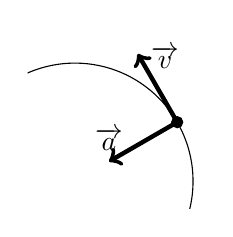
\begin{tikzpicture}[scale=0.5]

\clip (-1.2,-0.7) rectangle (3.30000,3.90000) ;

\coordinate (M) at (2.59808,1.50000) ;
\coordinate (O) at (0,0);

\draw (O) circle (3) ;

\filldraw [fill=black] (M) circle (4pt) ;

\draw [ultra thick,->,shift=(M)] (0,0) -- (-1.00000,1.73205) node [pos=0.95,right] {$\vect{v}$};

\draw [ultra thick,->] (M) -- (0.86603,0.50000) node [pos=1,above] {$\vect{a}$};

\end{tikzpicture}}

\def\ACCELERE{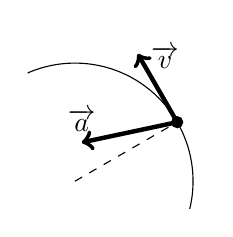
\begin{tikzpicture}[scale=0.5]

\clip (-1.2,-0.7) rectangle (3.30000,3.90000) ;

\coordinate (M) at (2.59808,1.50000) ;
\coordinate (O) at (0,0);

\draw (O) circle (3) ;

\filldraw [fill=black] (M) circle (4pt) ;

\draw [ultra thick,->,shift=(M)] (0,0) -- (-1.00000,1.73205) node [pos=0.95,right] {$\vect{v}$};

\draw [ultra thick,->] (M) -- (0.17365,0.98481) node [pos=1,above] {$\vect{a}$};
\draw [dashed] (O) -- (M) ;

\end{tikzpicture}}

\def\RALENTI{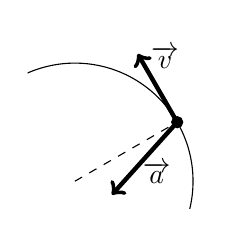
\begin{tikzpicture}[scale=0.5]

\clip (-1.2,-0.7) rectangle (3.30000,3.90000) ;

\coordinate (M) at (2.59808,1.50000) ;
\coordinate (O) at (0,0);

\draw (O) circle (3) ;

\filldraw [fill=black] (M) circle (4pt) ;

\draw [ultra thick,->,shift=(M)] (0,0) -- (-1.00000,1.73205) node [pos=0.95,right] {$\vect{v}$};

\draw [ultra thick,->] (M) -- (0.93969,-0.34202) node [pos=0.7,right] {$\vect{a}$};
\draw [dashed] (O) -- (M) ;

\end{tikzpicture}}


\hfil
\begin{animateinline}[autoplay,loop,controls]{10}
    \multiframe{36}{rangle=0+10}{
        \POLAIREUN{\rangle}
    }
\end{animateinline}\hfil
\begin{animateinline}[autoplay,loop,controls]{10}
    \multiframe{36}{rangle=0+10}{
        \POLAIREDEUX{\rangle}
    }
\end{animateinline}



\bk

\hfil\begin{animateinline}[autoplay,loop,controls]{10}
    \multiframe{36}{rangle=0+10}{
\begin{tikzpicture}[scale=6]

%% Les valeurs utiles

\ifthenelse{\rangle < 301}{
  \pgfmathsetmacro{\THETA}{60+\rangle}
}{
  \pgfmathsetmacro{\THETA}{\rangle-300}
}
\pgfmathsetmacro{\Z}{0.3+0.15*cos(\rangle)}
\pgfmathsetmacro{\coeff}{0.3}
\pgfmathsetmacro{\R}{0.3+0.2*cos(\rangle)}
\pgfmathsetmacro{\X}{\R*cos(\THETA)}
\pgfmathsetmacro{\Y}{\R*sin(\THETA)}
\pgfmathsetmacro{\UNIT}{0.15}

\coordinate (O)   at (0,0,0) ;
\coordinate (M) at (\Y,\Z,\X) ;
\coordinate (Mr) at ({\Y+\UNIT*sin(\THETA)},\Z,{\X+\UNIT*cos(\THETA)}) ;
\coordinate (Mt) at ({\Y+\UNIT*cos(\THETA)},\Z,{\X-\UNIT*sin(\THETA)}) ;
\coordinate (Mz) at (\Y,\Z+\UNIT,\X) ;
\coordinate (H) at (0,\Z,0) ;
\coordinate (P) at (\Y,0,\X) ;
\coordinate (Px) at (0,0,\X) ;
\coordinate (Py) at (\Y,0,0) ;
\coordinate (P1) at ($0.4*(P)$) ;
\coordinate (P1perp) at (0.4*\Y-0.3*0.4*\X,0,0.4*\X+0.3*0.4*\Y) ;
\coordinate (X) at (0,0,0.2) ;
\coordinate (Xperp) at (0.1,0,0.2) ;

%% Vecteurs
  \draw [->] (-0.2,0,0) -- (0.8,0,0) node [right] {$y$} ;
  \draw [->] (0,-0.2,0) -- (0,0.8,0) node [left] {$z$} ;
  \draw [->] (0,0,-0.2) -- (0,0,0.8) node [left] {$x$} ;
  \draw [ultra thick,->] (O) -- (M) node [pos=0.5,above left=-2pt] {$\vect{OM}$} ;
  \draw [ultra thick,->] (M) -- (Mr) node [right] {$\ver$} ;
  \draw [ultra thick,->] (M) -- (Mt) node [above right=-4pt] {$\vetheta$} ;
  \draw [ultra thick,->] (M) -- (Mz) node [right] {$\vez$} ;
  \draw [dashed] (O) -- (P) -- (M)   node [pos=0.5,right] {$z$}  ;
  \draw [dashed] (O) -- (H) node [left] {H} 
  		-- (M) node [pos=0.5, above] {$r$} ;
  \filldraw[black] (H) circle(0.3pt) ;
  \filldraw[black] (P) circle(0.3pt) node [below] {$P$};
  \filldraw[black] (O) circle(0.3pt) node [left] {$O$};
  \draw [dotted] (Px) -- (P) -- (Py) ;

%% Angle
%  \draw [thick,->] (X) .. controls (Xperp) and (P1perp) .. (P1)
%    node [below,pos=0.5] {$\theta$};
\draw [thick,->] (0,0,\UNIT) node [below right=-2pt] {$\theta$}
   \foreach \t in {0,10,...,\THETA} {
     -- ({\UNIT*sin(\t)},0,{\UNIT*cos(\t)})
   }
   ;


\end{tikzpicture}
}
\end{animateinline}


\bk

\hfil%% Les valeurs utiles


\begin{animateinline}[autoplay,loop,controls]{4}
    \multiframe{36}{rangle=0+10}{

\begin{tikzpicture}[scale=1.5]
\pgfsetzvec{\pgfpointxy{-0.30619}{-0.17678}}

\pgfmathsetmacro{\THETAr}{int(35+\rangle/2)}
\pgfmathsetmacro{\PHIr}{int(40+\rangle)}

\draw (0,0) -- (1,0) ;

%\ifthenelse{\THETAr<10}{Go}{RCS}

\ifthenelse{{\THETAr > 180}}{
  \pgfmathsetmacro{\THETA}{\THETAr-180}
}{
  \pgfmathsetmacro{\THETA}{\THETAr}
}



%\ifthenelse{\PHIr > 360}{
%  \pgfmathsetmacro{\PHI}{\PHIr - 360}
%}{
%  \pgfmathsetmacro{\PHI}{\PHIr}
%}

\pgfmathsetmacro{\PHI}{60*cos(2*\rangle)}



\pgfmathsetmacro{\R}{3}
\pgfmathsetmacro{\UNIT}{0.7}
\pgfmathsetmacro{\Z}{\R*cos(\THETA)}
\pgfmathsetmacro{\X}{\R*sin(\THETA)*cos(\PHI)}
\pgfmathsetmacro{\Y}{\R*sin(\THETA)*sin(\PHI)}


\coordinate (M) at (\Y,\Z,\X) ;
\coordinate (P) at (\Y, 0,\X) ;
\coordinate (H) at ( 0,\Z, 0) ;
\coordinate (O) at ( 0, 0, 0) ;
%\coordinate (Mr) at ({(M) + \UNIT*(-sin(\THETA)*sin(\PHI),cos(\THETA),sin(\THETA)*cos(\PHI))}) ;


%\clip  (-3.1,-0.7) rectangle (3.5,3.5);

%% Les axes

\draw [->,semithick] (-4.5,0,0) -- (4.5,0,0)  node [right] {$y$} ;
%\draw [semithick] ({\R*sin(-75)},0,{\R*cos(-75)}) -- ({-\R},0,{\R}) -- ({\R},0,{\R}) 
%	-- ({\R},0,{-\R}) -- ({-\R},0,{-\R}) ;
\draw [semithick] ({(\R)*sin(-75)*sin(75)},{(\R)*cos(75)},{(\R)*cos(-75)*sin(75)})
	-- ({-\R-1},0,{\R+1}) -- ({\R+1},0,{\R+1}) 
	-- ({\R+1},0,{-\R-1}) -- ({-\R-1},0,{-\R-1}) ;
\filldraw [white] (O) circle ({\R}) ;
%\draw [semithick] ({\R*sin(-75)},0,{\R*cos(-75)}) -- ({-\R},0,{\R}) -- ({\R},0,{\R}) 
%	-- ({\R},0,{-\R}) ;
\draw [semithick] 
	   ({-\R-1},0,{\R+1}) -- ({\R+1},0,{\R+1}) 
	-- ({\R+1},0,{-\R-1});
\draw [->,semithick] (0,-4,0) -- (0,3.5,0)  node [right] {$z$} ;

% Les diff�rents m�ridiens pour voir la sph�re
\foreach \p in {-75,-60,...,90} {
  \draw [dotted] (0,\R,0)
    \foreach \t in {0,10,...,160} {
        -- ({\R*sin(\t)*sin(\p)},{\R*cos(\t)},{\R*sin(\t)*cos(\p)}) 
    } ;
}

% Et les diff�rents parall�les
\foreach \t in {0,20,...,180} {
  \draw [dotted] ({\R*sin(\t)*sin(-70)},{\R*cos(\t)},{\R*cos(-70)*sin(\t)})
   \foreach \p in {-70,-60,...,90} {
        -- ({\R*sin(\t)*sin(\p)},{\R*cos(\t)},{\R*sin(\t)*cos(\p)}) 
   } ;
}

\pgfmathsetmacro{\t}{90}
  \draw ({\R*sin(\t)*sin(-70)},{\R*cos(\t)},{\R*cos(-70)*sin(\t)})
   \foreach \p in {-70,-60,...,90} {
        -- ({\R*sin(\t)*sin(\p)},{\R*cos(\t)},{\R*sin(\t)*cos(\p)}) 
   } ;


%\draw [dashed] (0,0,{-\R-1.5}) -- (0,0,\R) ; % x
\draw [dashed] (0,0,{0}) -- (0,0,\R) ; % x
%\draw [dashed] (0,{-\R},0) -- (0,\R,0) ; % z
%\draw [dashed] ({-\R},0,0) -- (\R,0,0) ; % y
\draw [->,semithick] (0,0,\R) -- (0,0,{\R+2})  node [below] {$x$} ;
%\draw [->] (\R,0,0) -- ({\R+0.5},0,0) node [above] {$y$} ;
%\draw [->] (0,\R,0) -- (0,{\R+0.5},0) node [right] {$z$} ;
%\draw ({-\R},0,0) -- ({-0.5-\R},0,0)
%      (0,{-\R},0) -- (0,{-0.5-\R},0) ;


% Le cercle


%\filldraw [thick, fill=gray] (O) -- (H) node [pos=0.5,left] {$r\cos\theta$} 
%		-- (M) 		
%		-- (P) -- (O) 
%		;
\draw [thick] (O) -- (H) %node [pos=0.5,\ifthenelse{\PHI>0}{left}{right}] {$r\cos\theta$} 
		-- (M) 		
		-- (P) -- (O) 
		;

%\draw [semithick,dotted] (0,0,\X) -- (P) -- (\Y,0,0) ;

\coordinate (Mi) at ($ 0.7*(P) + 0.3*(O)$);
\coordinate (Mib) at ($ (Mi) + (-0.2,-0.2) $);
\coordinate (Orig) at (2.5,-2.5) ;

\draw [<-] (Mi) .. controls (0,-1.5) and (1.5,0) .. (Orig)
		node [below=-3pt] {$ r\sin\theta$} ;

\draw [<-] (-0.1,{\Z/2}) .. controls (-1.5,0) and (0,1.5) .. (-2.5,2.5)
		node [above=-3pt] {$ r\cos\theta$} ;


% Position des points principaux
%  \filldraw[black] (M) circle(1pt) node [left] {$M$} ;
  \filldraw[black] (H) circle(1pt) node [left] {$H$} ;
  \filldraw[black] (P) circle(1pt) node [below] {$P$} ;

%% Les lignes d'angles
  \draw [ultra thick,->] (O) -- (M) node [pos=0.5,below] {$\quad r$};


%% Les ellipses des construction
    
% Le m�ridien d'abord
\draw [dashed,semithick] (0,\R,0)
    \foreach \t in {0,10,...,180} {
        -- ({\R*sin(\t)*sin(\PHI)},{\R*cos(\t)},{\R*sin(\t)*cos(\PHI)}) 
    } ;

% Le parall�le ensuite
\draw [dashed,semithick] ({-\R*sin(\THETA)*sin(70)},{\R*cos(\THETA)},{\R*cos(70)*sin(\THETA)})
   \foreach \p in {-70,-60,...,90} {
        -- ({\R*sin(\THETA)*sin(\p)},{\R*cos(\THETA)},{\R*sin(\THETA)*cos(\p)}) 
   } ;
    
%  \ELLIPSEUN
%%  \ELLIPSEDEUX
%  \ELLIPSETROIS
%%  \ELLIPSEQUATRE

%% Vecteurs
%\VER
\draw [->,ultra thick,shift={(M)}] (0,0,0) -- ({\UNIT*sin(\THETA)*sin(\PHI)},{\UNIT*cos(\THETA)},{\UNIT*sin(\THETA)*cos(\PHI)}) node [right] {$\ver$};
%\VETHETA
\draw [->,ultra thick,shift={(M)}] (0,0,0) -- ({\UNIT*cos(\THETA)*sin(\PHI)},{-\UNIT*sin(\THETA)},{\UNIT*cos(\THETA)*cos(\PHI)}) node [right] {$\vetheta$};
%\VEPHI
\draw [->,ultra thick,shift={(M)}] (0,0,0) -- ({\UNIT*cos(\PHI)},{0},{-\UNIT*sin(\PHI)}) node [right] {$\vephi$};

%  \draw (0,-3) -- (0,3) ;

%% Angles



%\THETA
{
\pgfmathsetmacro{\R}{1}
% Le m�ridien d'abord
\draw [->,thick] (0,\R,0)
    \foreach \t in {0,...,10} {
        -- ({\R*sin(\t*\THETA/10.0)*sin(\PHI)},{\R*cos(\t*\THETA/10.0)},{\R*sin(\t*\THETA/10.0)*cos(\PHI)}) 
    } ;
\draw ({\R*sin(\THETA/2)*sin(\PHI)},{\R*cos(\THETA/2)},{\R*sin(\THETA/2)*cos(\PHI)})
	node [above right=-2pt] {$\theta$};

%\PHI
% Le parall�le ensuite
\draw [->,thick] ({\R*sin(90)*sin(0)},{\R*cos(90)},{\R*cos(0)*sin(90)}) 
   \foreach \t in {0,...,10} {
        -- ({\R*sin(90)*sin(\PHI*\t/10.0)},{\R*cos(90)},{\R*sin(90)*cos(\PHI*\t/10.0)}) 
   } ;
\draw ({\R*sin(90)*sin(\PHI/2.0)},{\R*cos(90)},{\R*cos(\PHI/2)*sin(90)}) node [below=-2pt] {$\ph$} ;

}

\end{tikzpicture}
}
\end{animateinline}



\end{document}
